\section{\textbf{Comparison with Other Approaches}}

To assess how the AME approach compares with alternatives in the literature we utilize the same network dataset used by \citet{cranmer:etal:2016}. The reason we use the same dataset is because of the model specification issue that arises when using ERGMs. As \citet[p. 8]{cranmer:etal:2016} note, when using ERGMs scholars must model third order effects and ``must also specify them in a complete and correct manner'' or the model will be misspecified. Thus to avoid providing an incorrect specification when comparing ERGM with the AME we use the application that they constructed. 

Their application utilizes a cross-sectional network measuring whether an actor indicated that they collaborated with another during the policy design of the Swiss CO$_{2}$ act \citep{ingold:2008}.\footnote{This is a directed relational matrix as an actor $i$ can indicate that they collaborated with $j$ but $j$ may not have stated that they collaborated with $i$.} The Swiss government proposed this act in 1995 with the goal of undertaking a 10\% reduction in CO$_{2}$ emissions by 2012. The act was accepted in the Swiss Parliament in 2000 and implemented in 2008. \citet{ingold:2008}, and subsequent work by \citet{ingold:fischer:2014}, sought to determine what drives collaboration among actors trying to affect climate change policy. The set of actors included in this network are those that were identified by experts as holding an important position in Swiss climate policy.\footnote{For further details on the methodology utilized in choosing the set of actors see \citet{ingold:2008,ingold:fischer:2014}.} In total, \citet{ingold:2008} identifies 34 relevant actors: five state actors, eleven industry and business representatives, seven environmental NGOs and civil society organizations, five political parties, and six scientific institutions and consultants. 

\begin{figure}[ht]
	\centering
	\begin{tabular}{cc}
	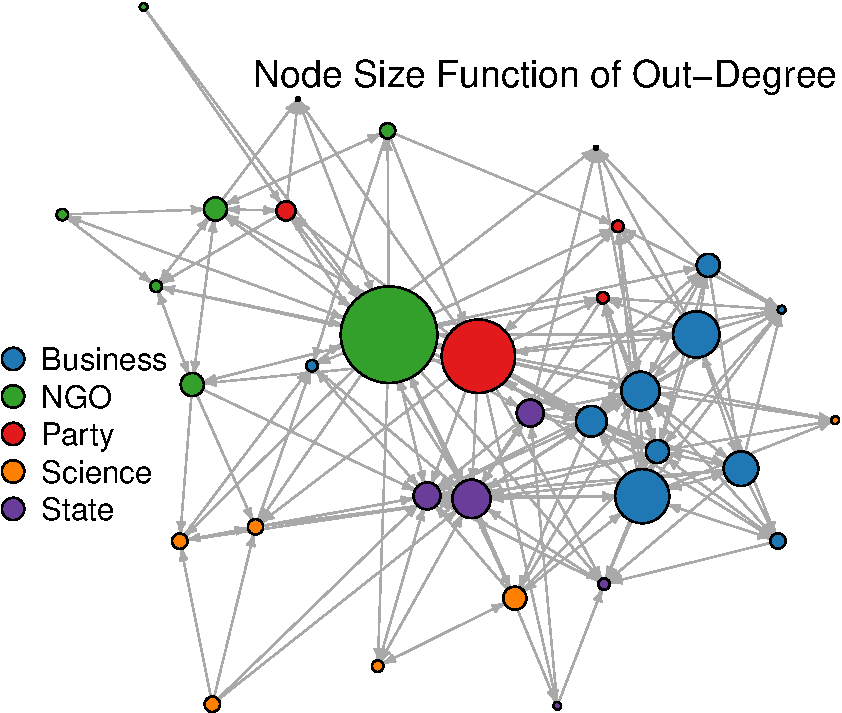
\includegraphics[width=.47\textwidth]{dvNet_outDegree} & 
	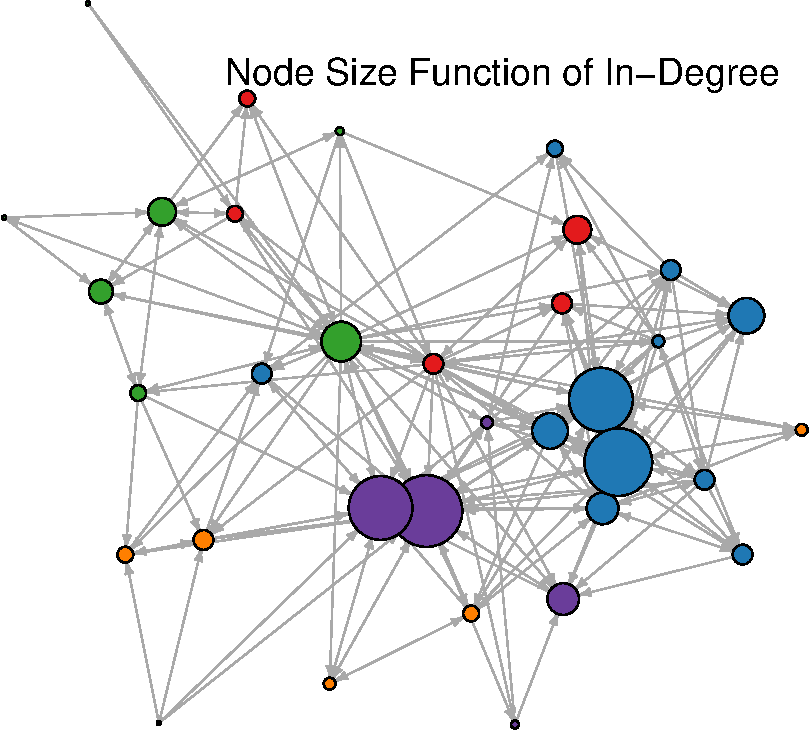
\includegraphics[width=.44\textwidth]{dvNet_inDegree}
	\end{tabular}
	\caption{Network visualizations of the Swiss climate change mitigation network. Nodes are colored by type of actor, and directed edges indicate relationships between actors. The network on the left weights node size by the number of out-going ties, and on the right the number of incoming-ties.}
	\label{fig:dvNet}
\end{figure}
\FloatBarrier

Figure~\ref{fig:dvNet} provides a pair of visualizations for this directed collaboration network. Nodes are colored by the type of actor and a directed edge indicates an actor stated that they collaborated with another, and determining which actor indicated the collaboration can be ascertained by the direction of the arrow. Actor positions are estimated using a force-directed layout algorithm.\footnote{To determine the positions of nodes in this network we use the Fruchterman-Reingold algorithm \citep{fruchterman:reingold:1991}. These types of algorithms use information contained within the structure of the network itself to construct depictions of graphs. A straightforward way to understand how they work is to think of nodes connected by edges as particles that are attracted to each other, and nodes that are unconnected as particles that repulse each other. These types of algorithms simulate a system in which nodes pull and push upon each other until they reach an equilibrium position.} Using this algorithm we see that the majority of industry and business actors are clustering together, meaning that these types of actors tend to indicate they collaborated with one another during the policy design process. We can also see that three of the state actors are pushed towards the center of the graph by the algorithm, which occurs because they share relationships with many actors in the network. Most of the actors classified as scientific institutions are pushed towards the far left border of the graphs as it seems they tend to interact amongst themselves and just a few of the other actors. 

An important part of our discussion from the previous section revolved around the idea that within network structures we find variation in how active nodes are in engaging with others in the network. To illustrate nodal heterogeneity in the case of the Swiss climate change mitigation networks we weight the size of nodes, in the network on the left, by the number of their outgoing ties, and on the right by their incoming ties. From the network on the left, it is clear that some nodes are much more likely to indicate that they formed collaborations with others. For example, each of the scientific institutions and consultants shown in Figure~\ref{fig:dvNet} indicate that they collaborate with relatively few organizations, especially, in comparison with actors from industry and business. Additionally, there is even variation within actor types as evidenced by differences amongst NGO or political party actors. Similar findings of nodal heterogeneity emerge if we turn our attention to examining nodes by their incoming ties. 

% The cursory discussion above regarding nodal heterogeneity should already point to the importance of taking into account lower order interdependencies between observations, and given the higher order structure  
Obvious from an examination of Figure~\ref{fig:dvNet} is that collaboration among these 34 actors is not simply a function of actor type. To understand what factors may play a role in shaping collaboration in this relational data structure a modeling approach is necessary, and based on our discussion from the previous section we would argue that a network analytic procedure is required. \citet{cranmer:etal:2016} follow \citet{ingold:fischer:2014} in developing a model specification. We do not review the specification in detail here, instead we just provide a summary of the variables to be included and the theoretical expectations of their effects in Table~\ref{tab:theorySpec}. 

\newcolumntype{L}{>{\arraybackslash}m{9cm}}
\begin{table}[ht]
\centering
\begingroup\scriptsize
\begin{tabular}{lLc}
\footnotesize{\textbf{Variable}} & \footnotesize{\textbf{Description}} & \footnotesize{\textbf{Expected Effect}} \\ \hline\hline
	\multicolumn{3}{l}{\textbf{Conflicting policy preferences}} \\ 
	\quad Business v. NGO & Binary, dyadic covariate that equals one when one actor is from the business sector and the other an NGO & $-$ \\
	\quad Opposition/alliance & Binary, dyadic covariate that equals one when $i$, sender, perceives $j$, receiver, as having similar policy objectives regarding climate change  & $+$ \\
	\quad Preference dissimilarity & Transformation of four core beliefs into a Manhattan distance matrix, smaller the distance the closer the beliefs of $i$ and $j$ & $-$ \\ 
	\multicolumn{3}{l}{\textbf{Transaction costs}} \\ 
	\quad Joint forum participation & Binary, dyadic covariate that equals one when $i$ and $j$ belong to the same policy forum & $+$ \\ 
	\multicolumn{3}{l}{\textbf{Influence}} \\ 
	\quad Influence attribution & Binary, dyadic covariate that equals one when $i$ considers $j$ to be influential & $+$ \\
	\quad Alter's influence in-degree & Number of actors that mention $i$ as being influential, this is a measure of reputational power & $+$ \\
	\quad Influence absolute diff. & Absolute difference in reputational power between $i$ and $j$ & $-$ \\
	\quad Alter = Government Actor & Binary, nodal covariate that equals one when $j$ is a state actor & $+$ \\ 
	\multicolumn{3}{l}{\textbf{Functional requirements}} \\ 
	\quad Ego = Environment NGO & Binary, nodal covariate that equals one when $i$ is an NGO & $+$ \\
	\quad Same actor type & Binary, dyadic covariate that equals when $i$ and $j$ are the same actor type & $+$ \\ 
	\multicolumn{3}{l}{\textbf{Endogenous dependencies: ERGM Specific Parameters}} \\ 
	\quad Mutuality & Captures concept of reciprocity, if $i$ indicates they collaborated with $j$ then $j$ likely collaborates with $i$ & $+$\\
	\quad Outdegree popularity & Captures idea that actors sending more ties will be more popular targets themselves for collaboration  & $+$ \\
	\quad Twopaths & Counts the number of two-paths in the network, two-path is an instance where $i$ is connected to $j$, $j$ to $k$, but $i$ is not connected to $k$ & $-$ \\
	\quad GWIdegree (2.0) & Takes into account how many ties a node sends in the network, used to capture network structures that result from some highly active nodes  & $+$ \\
	\quad GWESP (1.0) & Counts the number of shared partners for each pair and sums across  & $+$ \\
	\quad GWOdegree (0.5) & Takes into account how many ties a node receives in the network, used to capture networks structures that result from some highly popular nodes  & $+$ \\
\hline\hline
\end{tabular}
\endgroup
\caption{Summary of variables to be included in model specification. With the exception of mutuality, each of the parameters falling in the Endogenous dependencies grouping are only explicitly testable through ERGM. }
\label{tab:theorySpec}
\end{table}
\FloatBarrier

\subsection{Parameter Estimates}

Using the specification described in Table~\ref{tab:theorySpec} we compare five different modeling approaches. The first four approaches chosen here, as in \citet{cranmer:etal:2016}, are a logistic regression model, MRQAP, ERGM, and a latent space model (LSM) in which third order dependencies are accounted for via a two-dimensional Euclidean distance metric.\footnote{For a detailed discussion on the MRQAP see \citet{dekker:etal:2007}.} Parameter estimates for these four approaches are shown in Table~\ref{tab:regTable}. 

% latex table generated in R 3.3.1 by xtable 1.8-2 package
% Sun Aug 21 03:32:43 2016
\begin{table}[ht]
\centering
\begingroup\normalsize
\begin{tabular}{lccccc}
   & Logit & MRQAP & LSM & ERGM & AME \\ 
  \hline
\hline
Intercept/Edges & -4.44$^{\ast}$ & -4.24$^{\ast}$ & 0.94$^{\ast}$ & -12.17$^{\ast}$ & -3.39$^{\ast}$ \\ 
   & (0.34) &  & [0.09; 1.82] & (1.40) & [-4.38; -2.50] \\ 
  \textbf{Conflicting policy preferences} &  &  &  &  &  \\ 
  $\;\;\;\;$ Business vs. NGO & -0.86 & -0.87$^{\ast}$ & -1.37$^{\ast}$ & -1.11$^{\ast}$ & -1.37$^{\ast}$ \\ 
   & (0.46) &  & [-2.42; -0.41] & (0.51) & [-2.44; -0.47] \\ 
  $\;\;\;\;$ Opposition/alliance & 1.21$^{\ast}$ & 1.14$^{\ast}$ & 0.00 & 1.22$^{\ast}$ & 1.08$^{\ast}$ \\ 
   & (0.20) &  & [-0.40; 0.39] & (0.20) & [0.72; 1.47] \\ 
  $\;\;\;\;$ Preference dissimilarity & -0.07 & -0.60 & -1.76$^{\ast}$ & -0.44 & -0.79$^{\ast}$ \\ 
   & (0.37) &  & [-2.62; -0.90] & (0.39) & [-1.55; -0.08] \\ 
  \textbf{Transaction costs} &  &  &  &  &  \\ 
  $\;\;\;\;$ Joint forum participation & 0.88$^{\ast}$ & 0.75$^{\ast}$ & 1.51$^{\ast}$ & 0.90$^{\ast}$ & 0.92$^{\ast}$ \\ 
   & (0.27) &  & [0.86; 2.17] & (0.28) & [0.40; 1.47] \\ 
  \textbf{Influence} &  &  &  &  &  \\ 
  $\;\;\;\;$ Influence attribution & 1.20$^{\ast}$ & 1.29$^{\ast}$ & 0.08 & 1.00$^{\ast}$ & 1.09$^{\ast}$ \\ 
   & (0.22) &  & [-0.40; 0.55] & (0.21) & [0.69; 1.53] \\ 
  $\;\;\;\;$ Alter's influence indegree & 0.10$^{\ast}$ & 0.11$^{\ast}$ & 0.01 & 0.21$^{\ast}$ & 0.11$^{\ast}$ \\ 
   & (0.02) &  & [-0.03; 0.04] & (0.04) & [0.07; 0.15] \\ 
  $\;\;\;\;$ Influence absolute diff. & -0.03$^{\ast}$ & -0.06$^{\ast}$ & 0.04 & -0.05$^{\ast}$ & -0.07$^{\ast}$ \\ 
   & (0.02) &  & [-0.01; 0.09] & (0.01) & [-0.11; -0.03] \\ 
  $\;\;\;\;$ Alter = Government actor & 0.63$^{\ast}$ & 0.68 & -0.46 & 1.04$^{\ast}$ & 0.55 \\ 
   & (0.25) &  & [-1.08; 0.14] & (0.34) & [-0.07; 1.15] \\ 
  \textbf{Functional requirements} &  &  &  &  &  \\ 
  $\;\;\;\;$ Ego = Environmental NGO & 0.88$^{\ast}$ & 0.99 & -0.60 & 0.79$^{\ast}$ & 0.67 \\ 
   & (0.26) &  & [-1.32; 0.09] & (0.17) & [-0.38; 1.71] \\ 
  $\;\;\;\;$ Same actor type & 0.74$^{\ast}$ & 1.12$^{\ast}$ & 1.17$^{\ast}$ & 0.99$^{\ast}$ & 1.04$^{\ast}$ \\ 
   & (0.22) &  & [0.63; 1.71] & (0.23) & [0.63; 1.50] \\ 
  \textbf{Endogenous dependencies} &  &  &  &  &  \\ 
  $\;\;\;\;$ Mutuality & 1.22$^{\ast}$ & 1.00$^{\ast}$ &  & 0.81$^{\ast}$ & 0.39 \\ 
   & (0.21) &  &  & (0.25) & [-0.12; 0.96] \\ 
  $\;\;\;\;$ Outdegree popularity &  &  &  & 0.95$^{\ast}$ &  \\ 
   &  &  &  & (0.09) &  \\ 
  $\;\;\;\;$ Twopaths &  &  &  & -0.04$^{\ast}$ &  \\ 
   &  &  &  & (0.02) &  \\ 
  $\;\;\;\;$ GWIdegree (2.0) &  &  &  & 3.42$^{\ast}$ &  \\ 
   &  &  &  & (1.47) &  \\ 
  $\;\;\;\;$ GWESP (1.0) &  &  &  & 0.58$^{\ast}$ &  \\ 
   &  &  &  & (0.16) &  \\ 
  $\;\;\;\;$ GWOdegree (0.5) &  &  &  & 8.42$^{\ast}$ &  \\ 
   &  &  &  & (2.11) &  \\ 
   \hline
\hline
\end{tabular}
\endgroup
\caption{* p $<$ 0.05. Logistic regression and ERGM results are shown with standard errors in parentheses. MRQAP provides no standard errors. LSM and AME are shown with 95\% posterior credible intervals provided in brackets.} 
\label{tab:regTable}
\end{table}

\FloatBarrier

The fifth column shows the results from using the additive and multiplicative effects model (AME), in which we account for nodal and dyadic heterogeneity using the SRM and third order effects using a latent factor approach in which we set $K=2$.\footnote{Table~\ref{tab:regTable_ame} in Section~\ref{sec:ameVsAmeAppendix} of the Appendix shows that the parameter estimates presented here for the AME model remain very similar no matter the $K$ chosen. Additionally, trace plots for this model are shown in Figure~\ref{fig:ameConv} in the Appendix.} \citet{cranmer:etal:2016} provide a lengthy discussion of the differences between the first four modelling approaches that we will not repeat here. More relevant for us are how parameter estimates from AME relate to other approaches. The first point to note is that, in general, the parameter estimates returned by the AME are in many cases quite different from those returned by the LSM. For example, while the LSM returns a result for the \texttt{Opposition/alliance} variable that is quite different from MRQAP and ERGM, the AME returns a result that is not only similar to those approaches but in line with the theoretical expectations of \citet{ingold:fischer:2014}. Similar discrepancies between LSM and other approaches appear for parameters such as \texttt{Influence attribution} and \texttt{Alter's influence degree}. Each of these discrepancies are resolved when using AME. In part, this is a function of our discussion earlier about how the LSM approach as operationalized in the \pkg{latentnet} package can confound the effects of covariates with the latent space metric.\footnote{As shown in Table~\ref{tab:regTable_latSpace} in Section~\ref{sec:ameVsLatentnetAppendix} of the Appendix, these differences persist even when incorporating sender and receiver random effects or when switching to a bilinear approach to handle third order dependencies.}

There are also notable differences between the parameter estimates that result from the MRQAP, ERGM, and the AME. Using the AME we find evidence that \texttt{Preference dissimilarity} is associated with a reduced probability of collaboration between a pair of actors, which is in line with the theoretical expectations stated earlier. Additionally, the AME and MRQAP results differ from ERGM for the nodal effects related to whether a receiver of a collaboration is a government actor, \texttt{Alter=Government actor}, and whether the sender is an environmental NGO, \texttt{Ego=Environmental NGO}.

When it comes to estimating higher order effects, the logistic model and MRQAP are not able to provide information beyond an estimate of the effect of reciprocity, labeled as Mutuality in Table~\ref{tab:regTable}. ERGM is able to provide explicit estimates of a variety of higher order parameters, however, this comes with the caveat that these are the ``right'' set of endogenous dependencies. The AME approach, as shown in Equation~\ref{eqn:ame}, estimates network dependencies by examining patterns left over after taking into account the observed covariates. For the sake of space, we focus on examining the third order dependencies left over after accounting for the observed covariates and network covariance structure modeled by the SRM. A visualization of remaining third order dependencies is shown in Figure~\ref{fig:uv}. 

\begin{figure}[ht]
\centering
	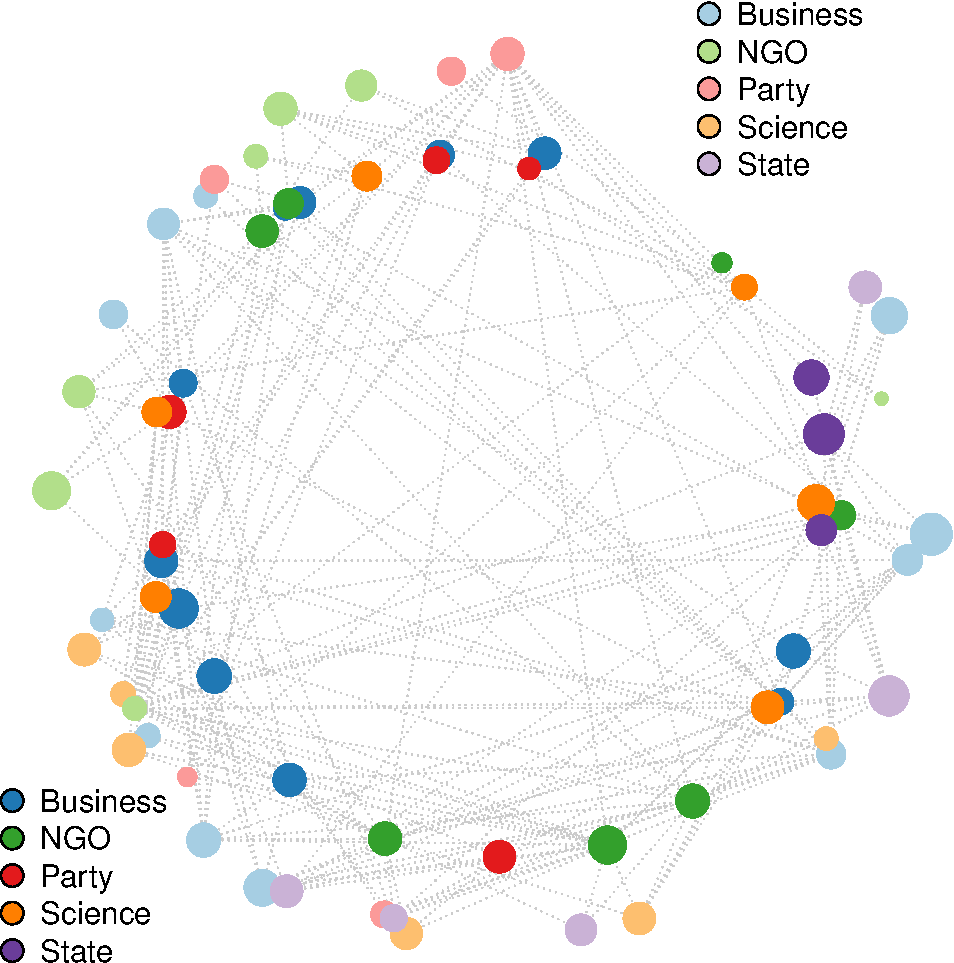
\includegraphics[width=.5\textwidth]{ameFitSR_2_UV}
	\caption{Circle plot of estimated latent factors.}
	\label{fig:uv}
\end{figure}
\FloatBarrier

In this figure, the directions of $\hat{u}_{i}$'s and $\hat{v}_{i}$'s are noted in lighter and darker shades, respectively, of an actor's type.\footnote{For example, actors from industry and business are assigned a color of blue and the direction of $\hat{u}_{i}$ for these actors is shown in light blue and $\hat{v}_{i}$ in dark blue} The size of actors is a function of the magnitude of the vectors, and dashed lines between actors indicate greater than expected levels of collaboration based on the regression term and additive effects. In the case of the application dataset that we are using here organization names have been anonymized and no additional covariate information is available. However, if we were to observe nodes sharing certain attributes clustering together in this circle plot that would mean such an attribute could be an important factor in helping us to understand collaborations among actors in this network. Given how actors of different types are distributed in almost a random fashion in this plot, we can at least be sure that it is unlikely other third order patterns can be picked up by that factor.

\subsection{Tie Formation Prediction}

Obviously an important test of any set of methods is how well they actually perform in terms of fitting the data. We provide a series of tests to assess model fit. First, are a set of diagnostics that are common in the political science literature. The left-most plot in Figure~\ref{fig:roc} compares the five approaches in terms of their ability to predict the in-sample occurrence of collaboration using Receiver Operating Characteristics (ROC) curves. ROC curves provide a comparison of the sensitivity and specificity trade-off for each model. Models that have a better fit according to this test should have curves that follow the left-hand border and then the top border of the ROC space. From this diagnostic it is clear that the AME model performs best in correctly predicting collaborations among actors in the Swiss climate change mitigation network. The LSM and ERGM approaches perform similarly and the MRQAP and Logit approaches fare notably worse.\footnote{Figure~\ref{fig:roc_latentSpace} in the Appendix provides additional comparisons between our AME approach and various parameterizations of the LSM, in each case we find that the AME approach provides far superior results in terms of predictive performance. Also important to note is that we can improve the fit of the AME model by increasing $K$ as shown in Figure~\ref{fig:roc_ame}. However, typically setting $K=2$ works well for most applied cases and choosing a $K$ higher than that increases the chances of overfitting the data.} 

\begin{figure}[ht]
	\centering
	\begin{tabular}{cc}
	\multicolumn{2}{c}{\textbf{In-Sample Performance}} \\
	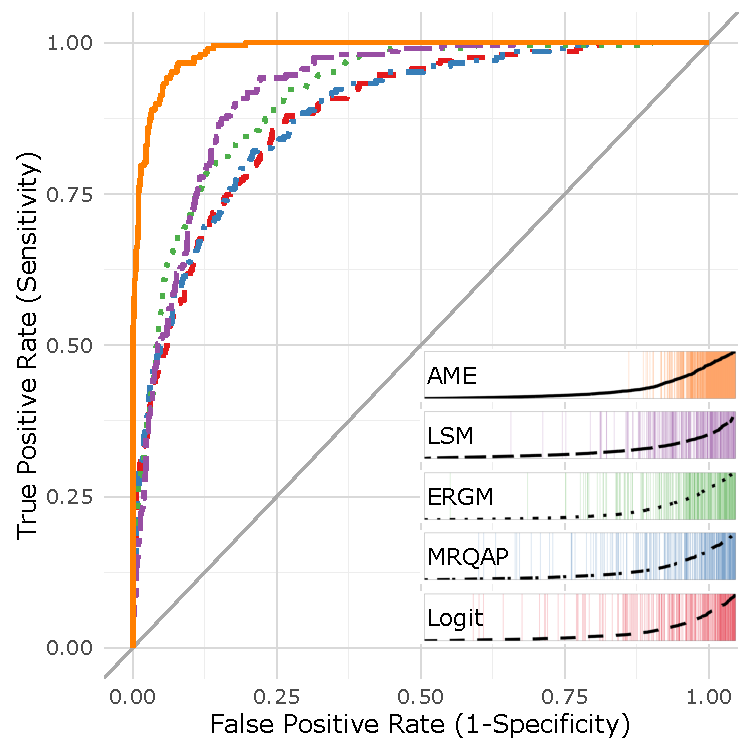
\includegraphics[width=.5\textwidth]{roc} & 
	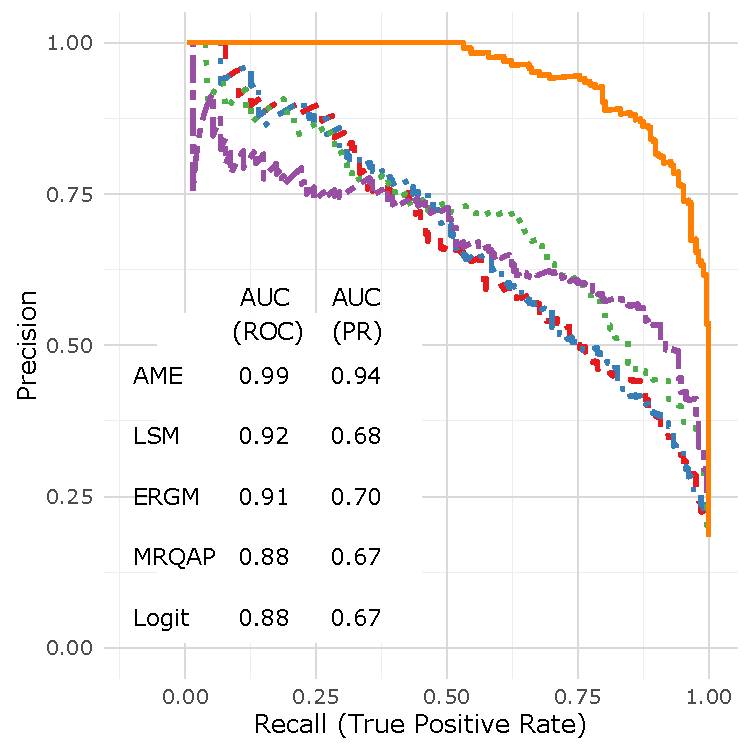
\includegraphics[width=.5\textwidth]{rocPr}	\\
	\multicolumn{2}{c}{\textbf{Out-of-Sample Performance}} \\	
	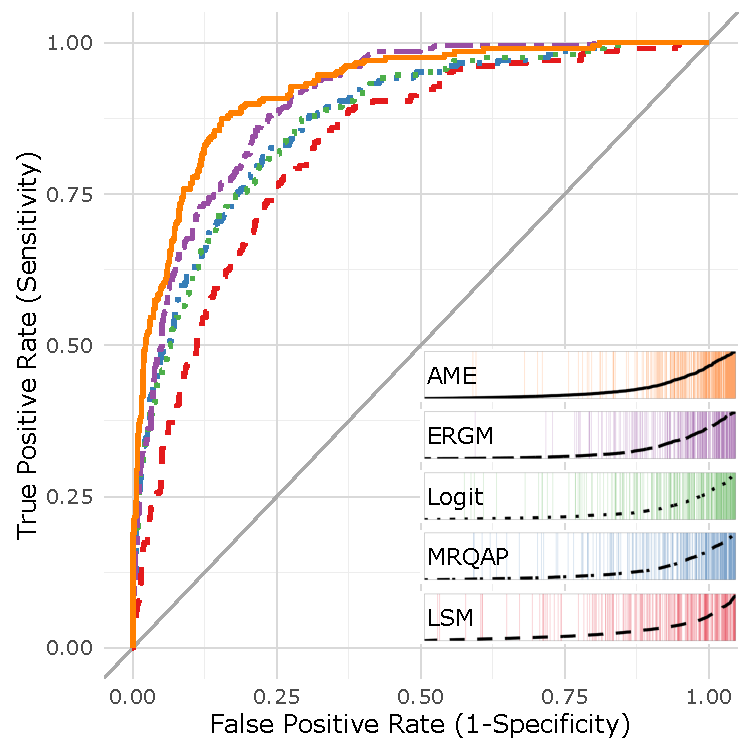
\includegraphics[width=.5\textwidth]{roc_outSample} & 
	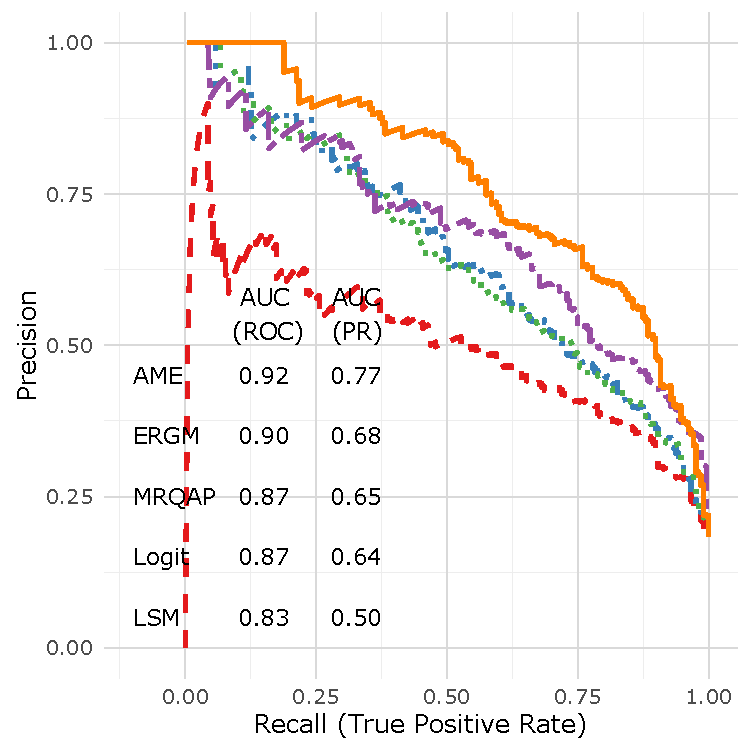
\includegraphics[width=.5\textwidth]{rocPr_outSample}	
	\end{tabular}
	\caption{Assessments of predictive performance using ROC curves, separation plots, and precision-recall curves. AUC statistics are provided as well for both the ROC and precision-recall curves. First row of plots provide assessments of in-sample fit, and second row out-of-sample fit.}
	\label{fig:roc}
\end{figure}
\FloatBarrier

A more intuitive visualization of the differences between these modeling approaches can be gleaned through examining the separation plots included on the right-bottom edge of the ROC plot \citep{greenhill:etal:2011}. This visualization tool plots each of the observations, in this case actor pairs, in the dataset according to their predicted value from left (low values) to right (high values). Models with a good fit should have all network links, here these are colored by the modeling approach, towards the right of the plot. Using this type of visualization we can again see that the AME model performs far better than the alternatives.

The last diagnostic we highlight to assess predictive performance are precision-recall curves. Precision is measure of relevancy that is calculated by taking the number of true positives over the total number of true and false positives. Recall is a measure of how many relevant results are returned and is calculated by taking the number of true positives over the number of true positives and false negatives. In this case, a curve will ideally follow the top boarder and then the right-hand border, when the curve for a model follows such a pattern this indicates that the model is returning both accurate (high precision) and a majority of all positive results (high recall). In this last diagnostic, we again find that the AME approach performs far better than alternatives, and that the other models are indistinguishable from one another in terms of performance. Area under the curve (AUC) statistics are also provided in Figure~\ref{fig:roc}.

\subsection{Capturing Network Attributes}

Now, in addition to the typical performance analyses presented in the previous section, for network data it is also important to assess whether a model adequately captures the network parameters of the dependent variable \citep{hunter:etal:2008}. To do this one can compare the observed network with a set of networks simulated from the estimated models. Below we show a standard set of parameters upon which comparisons are usually conducted:\footnote{See \citet{morris:etal:2008} for details on each of these parameters. If one was to examine goodness of fit in the \pkg{ergm} package these parameters would be calculated by default.}

\newcolumntype{L}{>{\arraybackslash}m{9cm}}
\begin{table}[ht]
\centering
\begingroup\scriptsize
\begin{tabular}{lL}
\footnotesize{\textbf{Variable}} & \footnotesize{\textbf{Description}} \\ \hline\hline
	Dyad-wise shared partners & Number of dyads in the network with exactly $i$ shared partners \\
	Edge-wise shared partners & Similar to above except this counts the number of dyads with the same number of edges \\
	Geodesic distances & The proportion of pairs of nodes whose shortest connecting path is of length $k$, for $k=1,2,\ldots$ Also, pairs of nodes that are not connected are classified as $k=\infty$ \\
	Incoming k-star & Propensities for individuals to have connections with multiple network partners \\
	Indegree & Degree count is the number of nodes with the same value of the attribute as the receiving node \\
	Outdegree & Degree count is the number of nodes with the same value of the attribute as the sending node \\
\hline\hline
\end{tabular}
\endgroup
\caption{Description of a set of standard statistics used to assess whether a model captures network dependencies. }
\label{tab:netStat}
\end{table}
\FloatBarrier

Given the already poor predictive performance that the Logit and MRQAP models exhibited in the previous section we exclude them from this next analysis. Instead we restrict our focus to the three approaches -- LSM, ERGM, and AME -- that explicitly seek to model network interdependencies. 

\begin{figure}[ht]
	\centering
	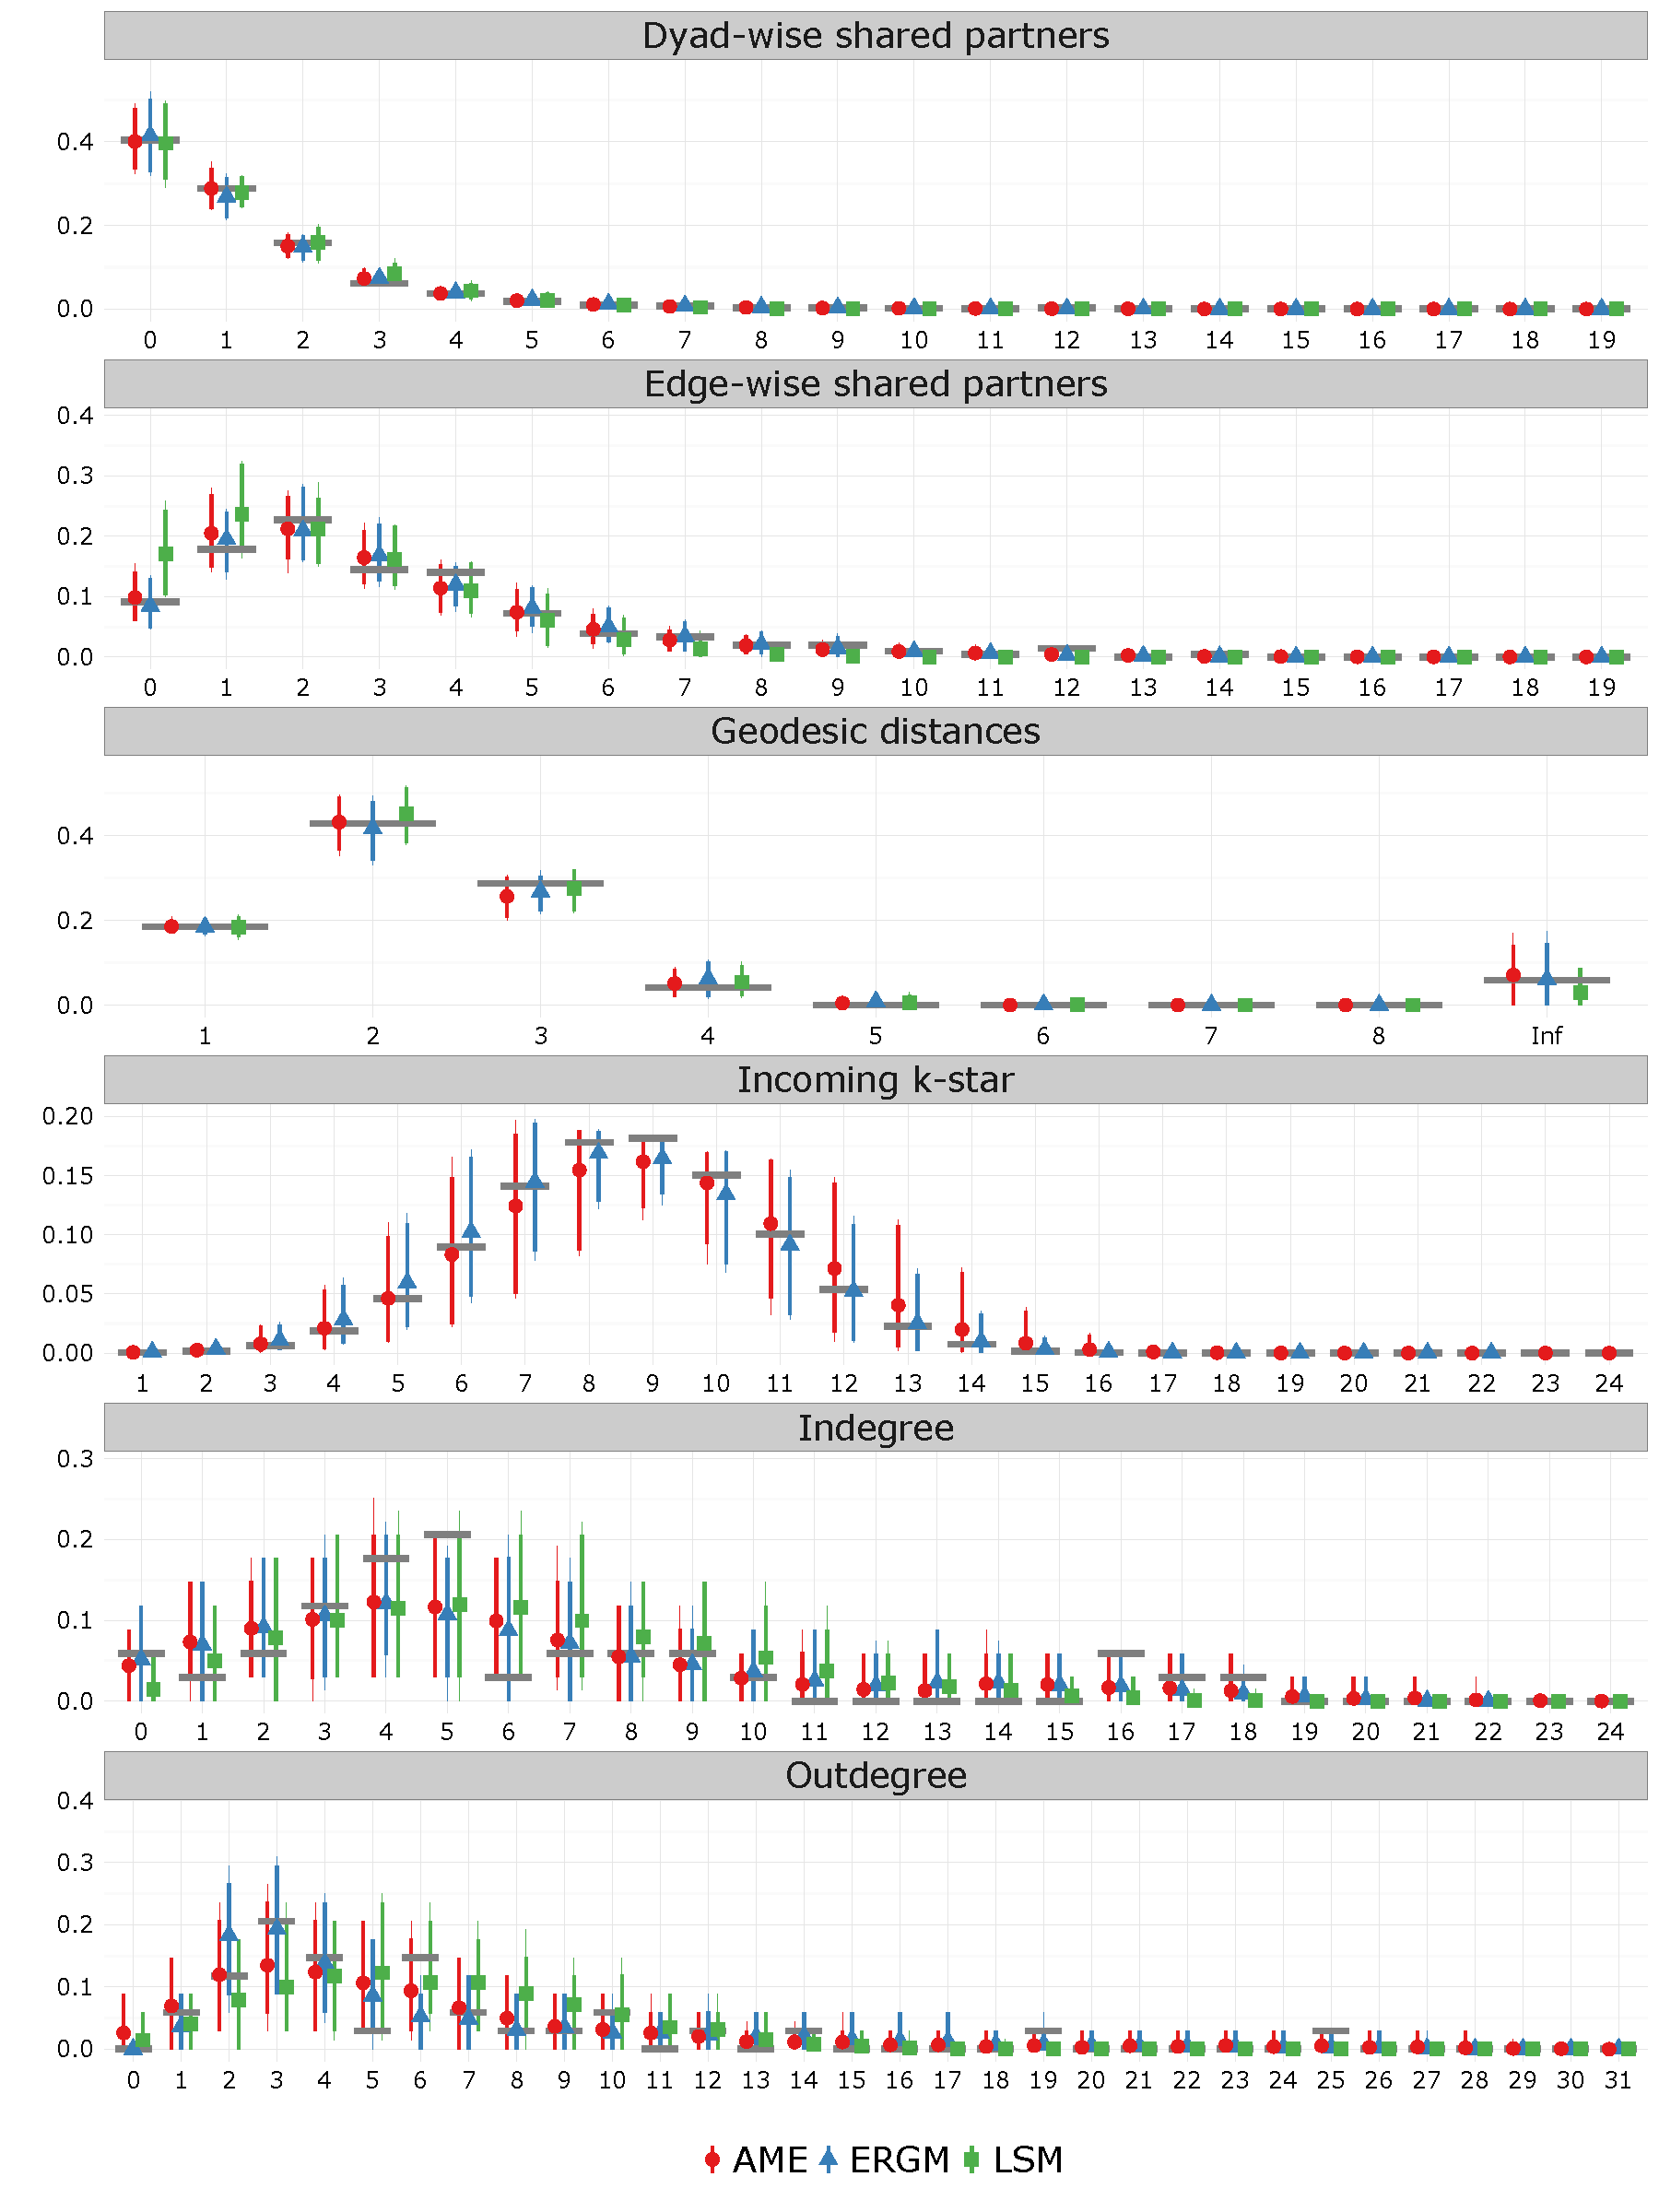
\includegraphics[width=1\textwidth]{ggGofAll}
	\caption{Goodness of fit statistics to assess how well the LSM, ERGM, and AME approaches account for network dependencies.}
	\label{fig:gofAll}
\end{figure}
\FloatBarrier

To run this analysis we simulate 1,000 networks from the three models, and we compare how well the simulated networks align with the observed network in terms of the statistics described in Table~\ref{tab:netStat}. The results of this analysis are shown in Figure~\ref{fig:gofAll}. Values for the observed network are indicated by a gray bar and average values from the simulated networks for the AME, ERGM, and LSM are represented by a diamond, triangle, and square, respectively. The densely shaded interval around each point represents the 95\% interval from the simulations and the taller, less dense the 90\% interval.\footnote{Calculation for the incoming k-star statistic is not currently supported by the \pkg{latentnet} package.} 

Looking across the panels in Figure~\ref{fig:gofAll} it is clear that there is little difference between the ERGM and AME models in terms of how well they capture network dependencies. The LSM model, however, does perform somewhat worse in comparison. Particularly, when it comes to assessing the number of edge-wise shared partners and in terms of capturing the indegree and outdegree distributions of the collaboration network. 

This becomes clearer when examining a more parsimonious set of diagnostics that are available in the \pkg{amen} package for assessing network goodness of fit using the same simulation based methodology. Specifically, \pkg{amen} provides goodness of fit summaries for four network statistics: (1) the empirical standard deviation of the row means (i.e., heterogeneity of nodes in terms of the ties they send); (2) the empirical standard deviation of the column means (i.e., heterogeneity of nodes in terms of the ties they receive); (3) the empirical within-dyad correlation (i.e., measure of reciprocity in the network); and (4) a normalized measure of triadic dependence \citep{hoff:etal:2015}. A comparison of the LSM, ERGM, and AME models among these four statistics is shown in Figure~\ref{fig:ergmAmePerf}.

\begin{figure}[ht]
	\centering
	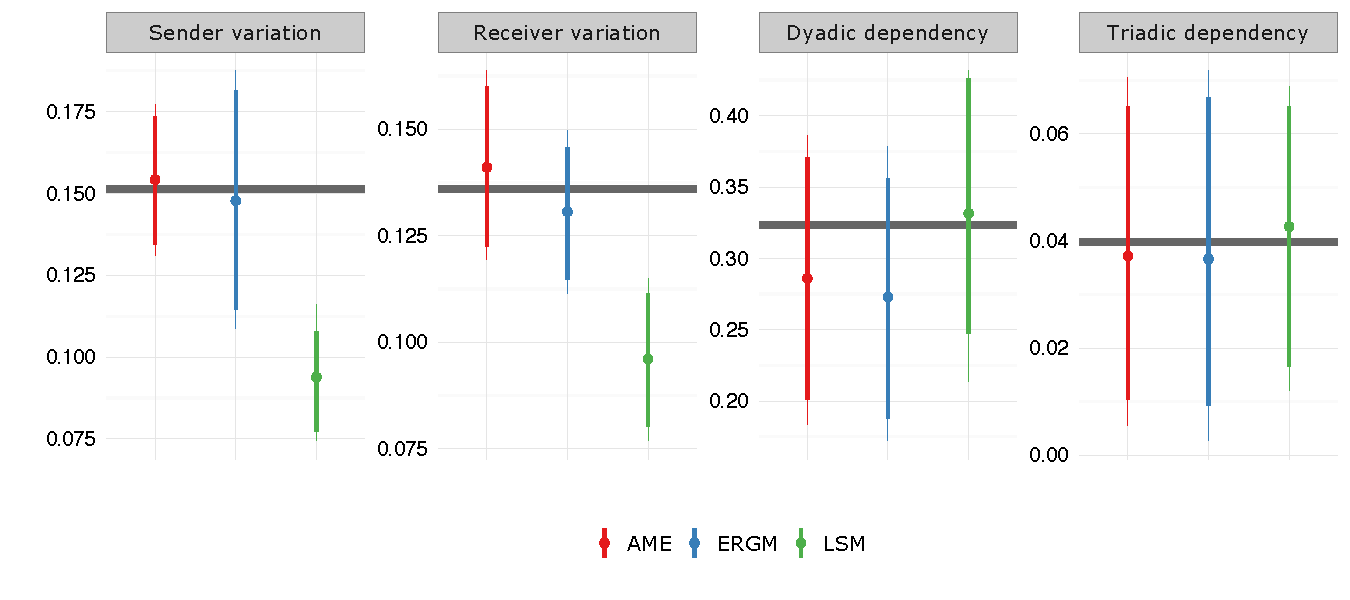
\includegraphics[width=1\textwidth]{netPerfCoef}
	\caption{Network goodness of fit summary using \pkg{amen}.}
	\label{fig:ergmAmePerf}
\end{figure}
\FloatBarrier

Here it becomes quickly apparent that the LSM model fails to capture how active and popular actors are in the Swiss climate change mitigation network.\footnote{Interestingly, even after incorporating random sender and receiver effects into the LSM framework this problem is not completely resolved, see Figure~\ref{fig:netPerfCoef_latSpace} in the Appendix for details.} The AME and ERGM specifications again both tend to do equally well.\footnote{Not surprisingly, if we increase $K$ in the AME approach we are able to better account for triadic dependencies, see Figure~\ref{fig:netPerfCoef_ameSR} in the Appendix for details.} If when running this diagnostic, we found that the AME model did not adequately represent the observed network this would indicate that we might want to increase $K$ to account for network interdependencies. No changes to the model specification as described by the exogenous covariates a researcher has chosen would be necessary. Now if the ERGM results do not align with the diagnostic presented in Figure~\ref{fig:ergmAmePerf} then this would indicates that an incorrect set of endogenous dependencies have been specified, failing to find the right specification will leave the researcher with the problems we introduced in the beginning of this paper.

% Simulating from ame mod
% For a given summary statistic g() we first simulate $\mathbf{Y}_{sim} \approx p(\mathbf{Y}_{sim} | \mathbf{Y}_{obs}) = \int p(\mathbf{Y}_{sim} | \theta) p(d \theta | \mathbf{Y}_{obs})$ and then we compare $g(\mathbf{Y}_{sim})$ to $g(\mathbf{Y}_{obs})$. Histograms represent predicted value of statistics under the model and red dash line represents the observed value. 

% Dyadic dep calc
% \begin{align}
% \begin{aligned}
% t(Y) &= \frac{ \sum_{i \neq j}y_{i,j} y_{j,i} }{ \sum_{i \neq j} y_{i,j} } \\
% \end{aligned}
% \end{align}

% Triadic dep assess
% \begin{align}
% \begin{aligned}
% t(Y) &= \sum_{i \neq j \neq k} y_{i,j} y_{i,k} y_{j,k}
% \end{aligned}
% \end{align}